% Options for packages loaded elsewhere
\PassOptionsToPackage{unicode}{hyperref}
\PassOptionsToPackage{hyphens}{url}
%
\documentclass[
  ignorenonframetext,
]{beamer}
\usepackage{pgfpages}
\setbeamertemplate{caption}[numbered]
\setbeamertemplate{caption label separator}{: }
\setbeamercolor{caption name}{fg=normal text.fg}
\beamertemplatenavigationsymbolsempty
% Prevent slide breaks in the middle of a paragraph
\widowpenalties 1 10000
\raggedbottom
\setbeamertemplate{part page}{
  \centering
  \begin{beamercolorbox}[sep=16pt,center]{part title}
    \usebeamerfont{part title}\insertpart\par
  \end{beamercolorbox}
}
\setbeamertemplate{section page}{
  \centering
  \begin{beamercolorbox}[sep=12pt,center]{part title}
    \usebeamerfont{section title}\insertsection\par
  \end{beamercolorbox}
}
\setbeamertemplate{subsection page}{
  \centering
  \begin{beamercolorbox}[sep=8pt,center]{part title}
    \usebeamerfont{subsection title}\insertsubsection\par
  \end{beamercolorbox}
}
\AtBeginPart{
  \frame{\partpage}
}
\AtBeginSection{
  \ifbibliography
  \else
    \frame{\sectionpage}
  \fi
}
\AtBeginSubsection{
  \frame{\subsectionpage}
}
\usepackage{amsmath,amssymb}
\usepackage{iftex}
\ifPDFTeX
  \usepackage[T1]{fontenc}
  \usepackage[utf8]{inputenc}
  \usepackage{textcomp} % provide euro and other symbols
\else % if luatex or xetex
  \usepackage{unicode-math} % this also loads fontspec
  \defaultfontfeatures{Scale=MatchLowercase}
  \defaultfontfeatures[\rmfamily]{Ligatures=TeX,Scale=1}
\fi
\usepackage{lmodern}
\ifPDFTeX\else
  % xetex/luatex font selection
\fi
% Use upquote if available, for straight quotes in verbatim environments
\IfFileExists{upquote.sty}{\usepackage{upquote}}{}
\IfFileExists{microtype.sty}{% use microtype if available
  \usepackage[]{microtype}
  \UseMicrotypeSet[protrusion]{basicmath} % disable protrusion for tt fonts
}{}
\makeatletter
\@ifundefined{KOMAClassName}{% if non-KOMA class
  \IfFileExists{parskip.sty}{%
    \usepackage{parskip}
  }{% else
    \setlength{\parindent}{0pt}
    \setlength{\parskip}{6pt plus 2pt minus 1pt}}
}{% if KOMA class
  \KOMAoptions{parskip=half}}
\makeatother
\usepackage{xcolor}
\newif\ifbibliography
\usepackage{graphicx}
\makeatletter
\def\maxwidth{\ifdim\Gin@nat@width>\linewidth\linewidth\else\Gin@nat@width\fi}
\def\maxheight{\ifdim\Gin@nat@height>\textheight\textheight\else\Gin@nat@height\fi}
\makeatother
% Scale images if necessary, so that they will not overflow the page
% margins by default, and it is still possible to overwrite the defaults
% using explicit options in \includegraphics[width, height, ...]{../figures/}
\setkeys{Gin}{width=\maxwidth,height=\maxheight,keepaspectratio}
% Set default figure placement to htbp
\makeatletter
\def\fps@figure{htbp}
\makeatother
\setlength{\emergencystretch}{3em} % prevent overfull lines
\providecommand{\tightlist}{%
  \setlength{\itemsep}{0pt}\setlength{\parskip}{0pt}}
\setcounter{secnumdepth}{-\maxdimen} % remove section numbering
% Slide layout defaults for warning-clean scientific decks.
\usepackage{etoolbox}
\IfFileExists{xurl.sty}{\usepackage{xurl}}{}
\IfFileExists{seqsplit.sty}{\usepackage{seqsplit}}{\newcommand{\seqsplit}[1]{#1}}
\protected\def\breakseq#1{\seqsplit{#1}}
\protected\def\breaktt#1{\begingroup\ttfamily\seqsplit{#1}\endgroup}
\setlength{\emergencystretch}{6em}
\tolerance=5000
\hbadness=10000
\hfuzz=1pt
\setlength{\tabcolsep}{2pt}
\AtBeginEnvironment{longtable}{\tiny\renewcommand{\arraystretch}{0.86}\setlength{\tabcolsep}{1pt}}
\AtBeginEnvironment{tabular}{\tiny\renewcommand{\arraystretch}{0.86}\setlength{\tabcolsep}{1pt}}

% Natbib and cross-reference fallbacks — slides don't load natbib
% or cleveref, but combined-PDF manuscript prose may emit these
% commands. The fallback renders citations as a bracketed key list
% and cross-references as detokenized labels so slides don't fail on
% undefined control sequences or raw underscores. \providecommand is
% a no-op if packages load later.
\providecommand{\citep}[1]{[#1]}
\providecommand{\citet}[1]{#1}
\providecommand{\citealp}[1]{#1}
\providecommand{\citeauthor}[1]{#1}
\providecommand{\citeyear}[1]{#1}
\providecommand{\cref}[1]{\texttt{\detokenize{#1}}}
\providecommand{\Cref}[1]{\texttt{\detokenize{#1}}}

\newtheorem{proposition}{Proposition}
\newtheorem{hypothesis}{Hypothesis}
\ifLuaTeX
  \usepackage{selnolig}  % disable illegal ligatures
\fi
\usepackage{bookmark}
\IfFileExists{xurl.sty}{\usepackage{xurl}}{} % add URL line breaks if available
\urlstyle{same}
\hypersetup{
  hidelinks,
  pdfcreator={LaTeX via pandoc}}

\author{}
\date{}

\begin{document}

\section{Results: Language, Topics, and
Embeddings}\label{results-language-topics-and-embeddings}

\begin{frame}[allowframebreaks]{RQ3: Topical and Linguistic Structure}
\phantomsection\label{rq3-topical-and-linguistic-structure}
Text analysis operates over titles, abstracts, and (when available) full
text. A TF-IDF representation over a
\{\{NUM\_VOCAB\_FEATURES\}\}-feature vocabulary feeds non-negative
matrix factorization, which extracts \{\{NUM\_TOPICS\}\} latent topics
cross-cutting the subfield taxonomy. The top vocabulary terms are:
\{\{TOP\_VOCAB\_TERMS\}\}.

\textbf{Table 3. NMF topics extracted from the corpus.}

\{\{TOPIC\_TABLE\}\}

The topic labels are computed from the retained corpus and are not
hand-assigned. Their interpretation should be checked against the
generated topic-term weights and the configured subfield taxonomy;
fixture-derived topics describe synthetic text patterns, not the
scientific field.

\begin{figure}
\centering
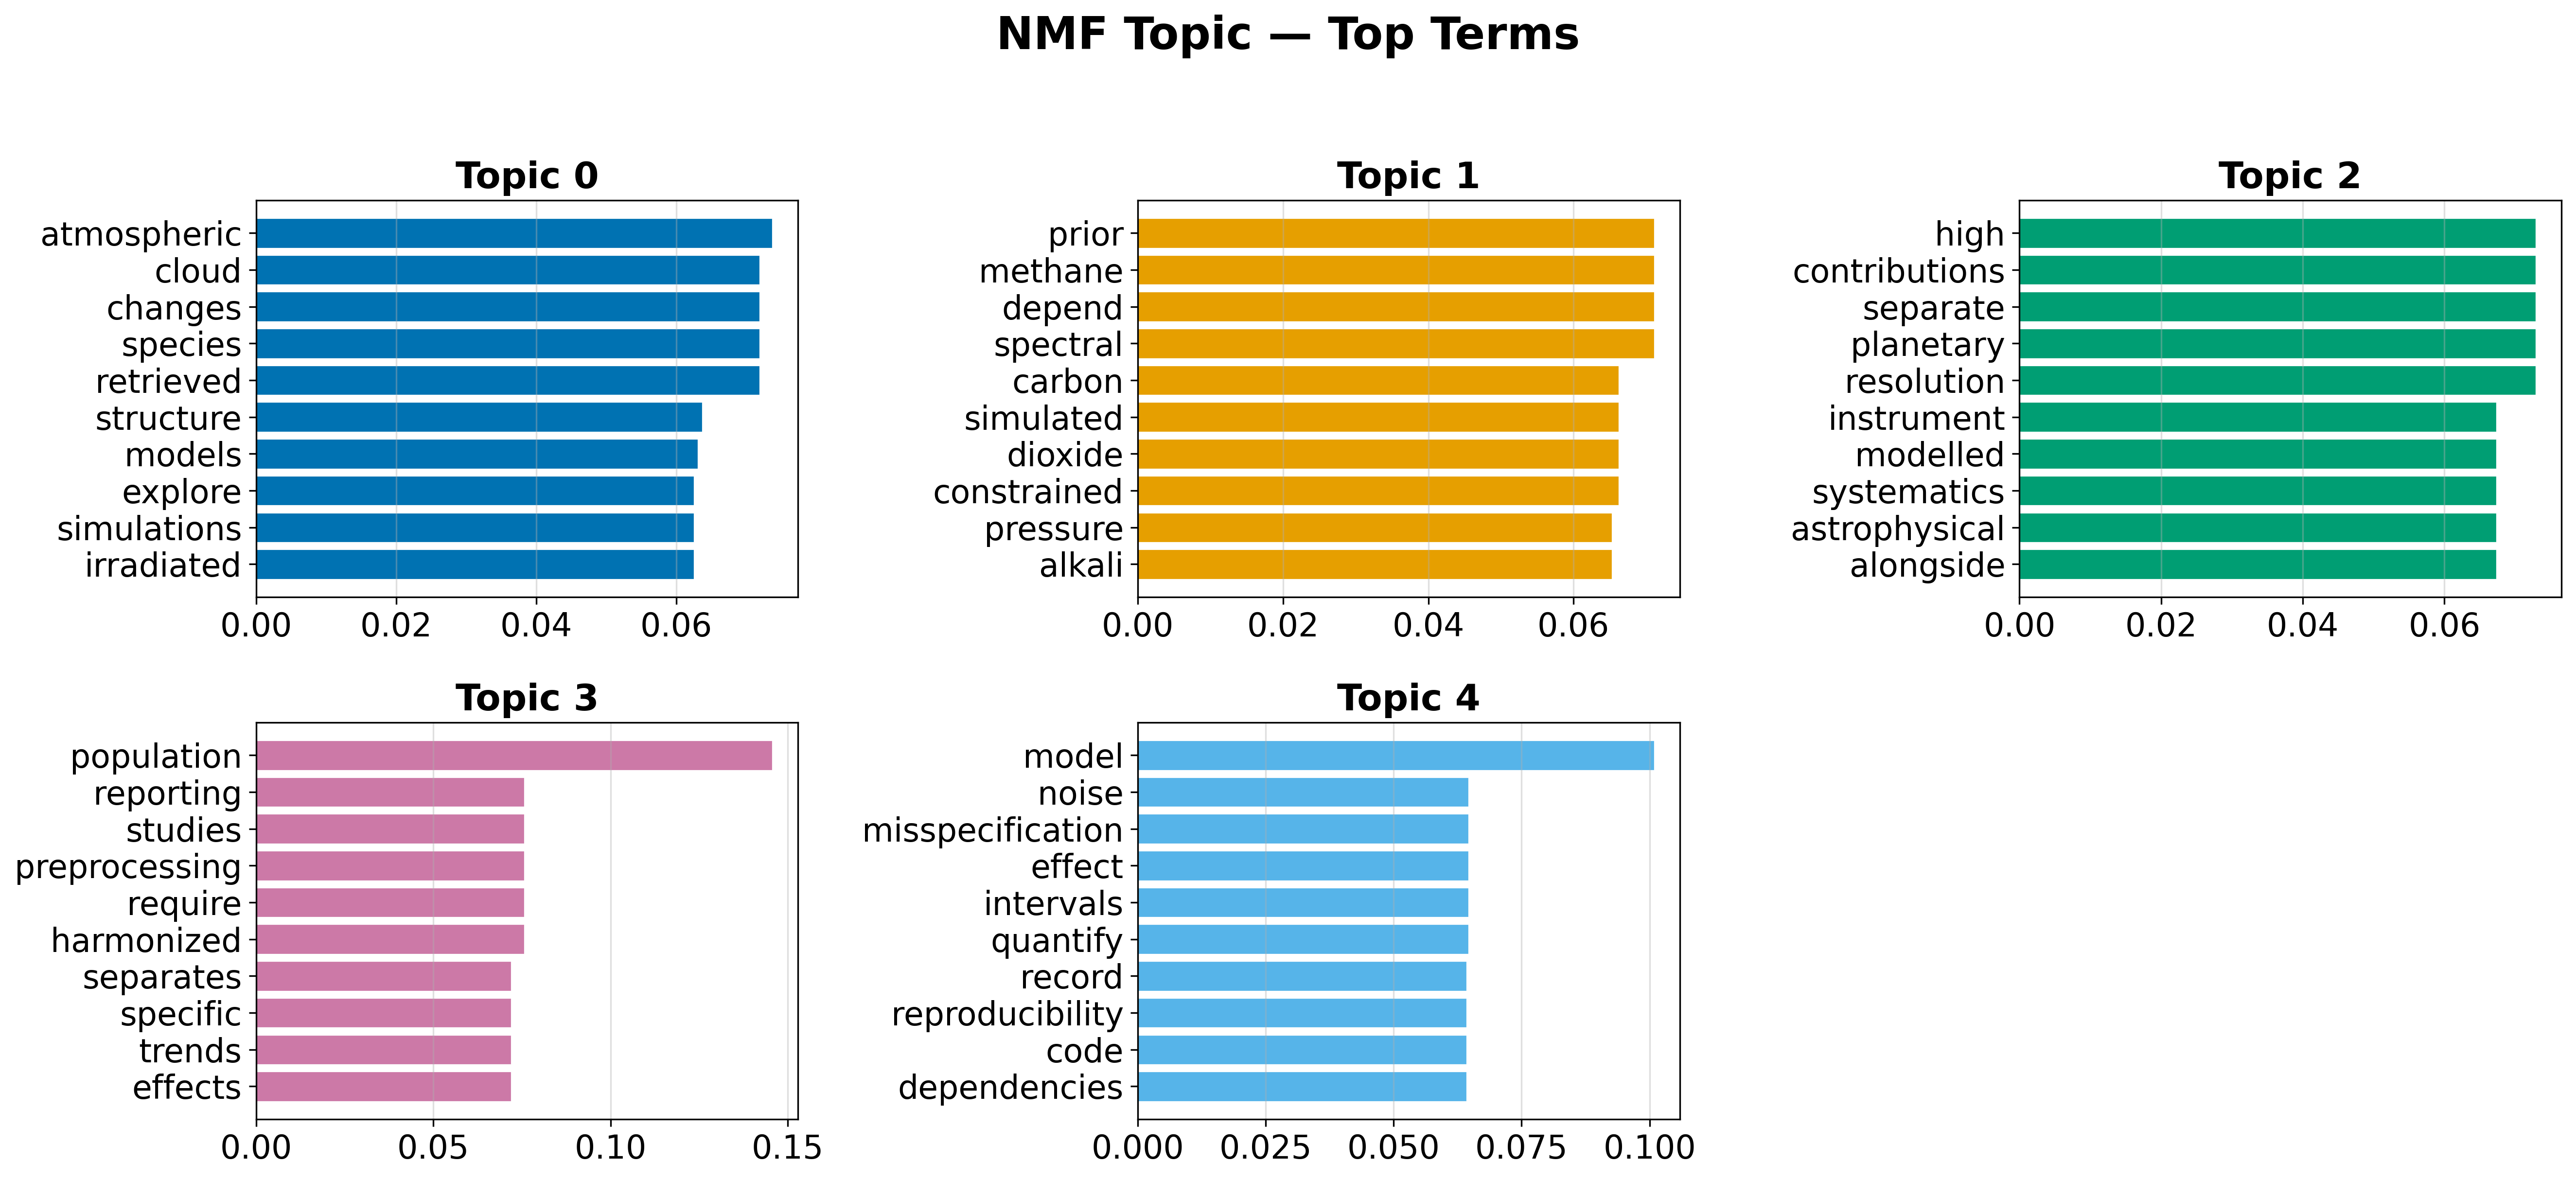
\includegraphics{../figures/topic_term_bars.png}
\caption{Topic-term bar charts for \{\{SEARCH\_TERM\_TITLE\}\}. Each
panel shows the top weighted terms for one of \{\{NUM\_TOPICS\}\} NMF
topics, with bar length proportional to the topic-term weight in the
\(\mathbf{H}\) matrix.}\label{fig:topic_term_bars}
\end{figure}
\end{frame}

\begin{frame}[allowframebreaks]{Document Embeddings}
\phantomsection\label{document-embeddings}
Offline deterministic embeddings (TF-IDF followed by truncated SVD)
place every document in a shared 50-dimensional vector space. Embedding
the same text twice yields identical vectors, so the derived similarity
matrix, nearest-neighbour lists, clusters, and two-dimensional
projection are all reproducible.

\begin{figure}
\centering
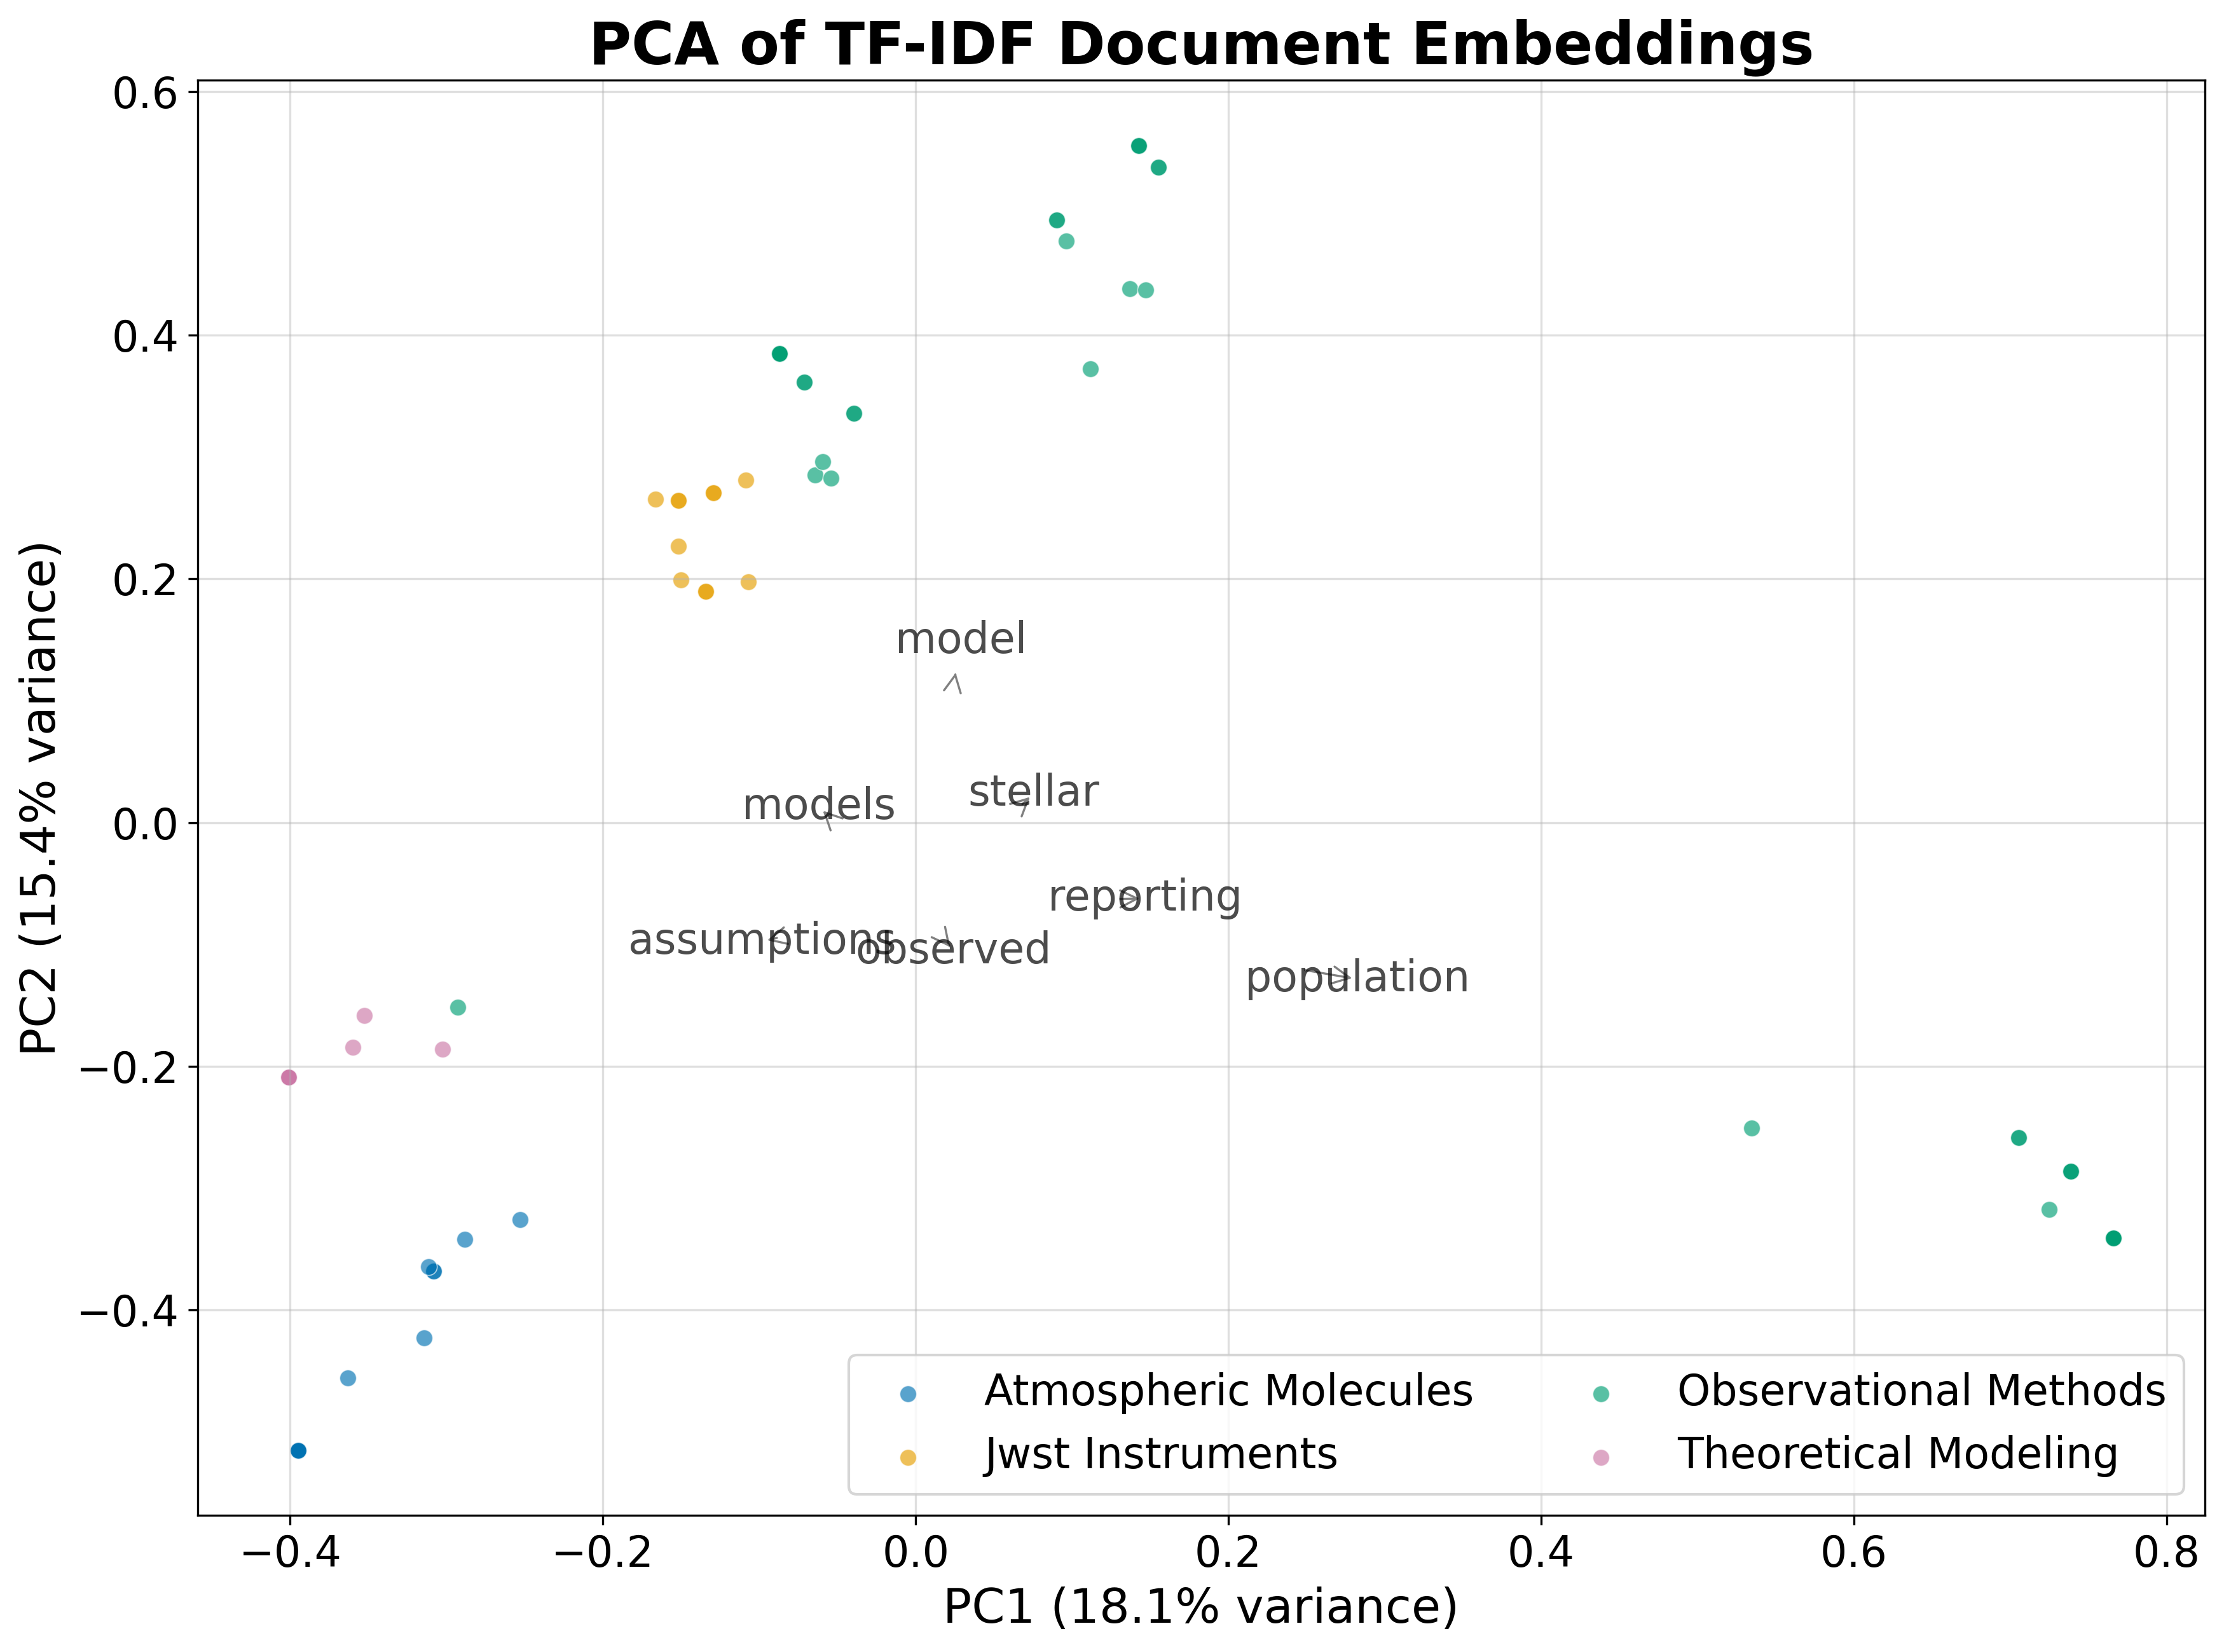
\includegraphics{../figures/pca_embeddings.png}
\caption{PCA projection of document embeddings for
\{\{SEARCH\_TERM\_TITLE\}\}. Each point represents one document
projected onto the first two principal components of the TF-IDF/SVD
embedding. Colours indicate subfield assignment, showing how the topical
geography relates to the keyword taxonomy.}\label{fig:pca_embeddings}
\end{figure}

\begin{figure}
\centering
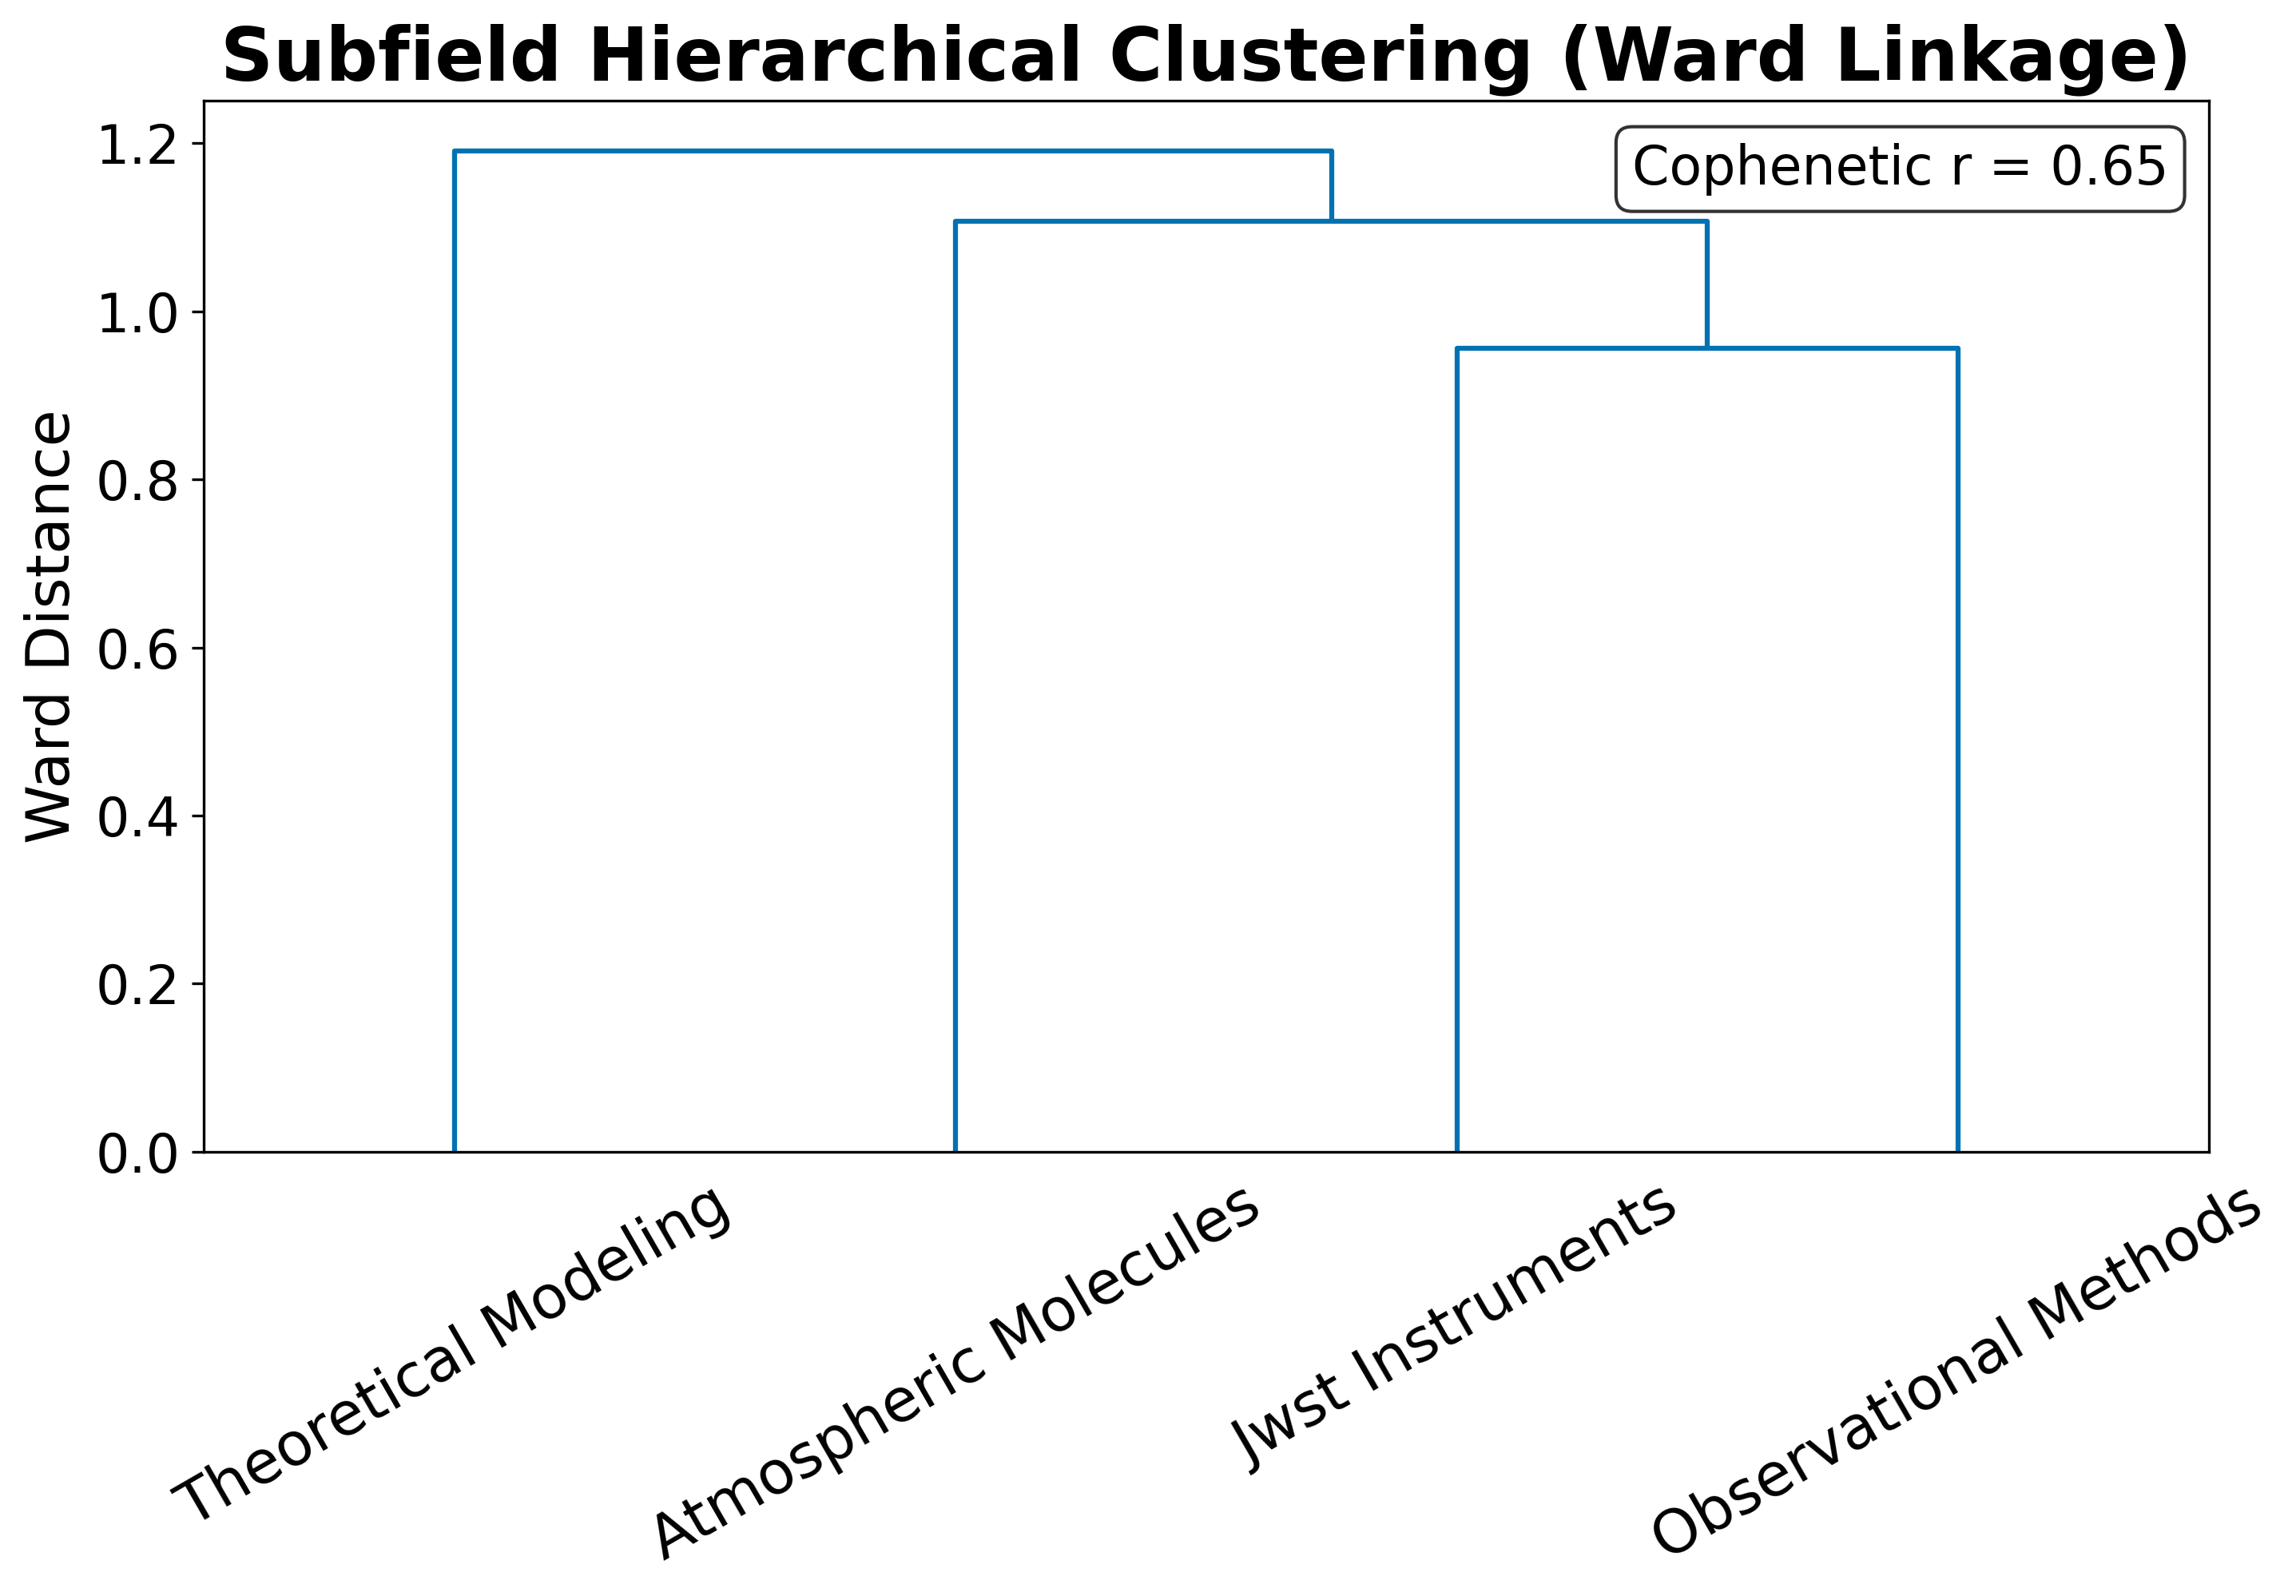
\includegraphics{../figures/dendrogram.png}
\caption{Hierarchical clustering dendrogram of document embeddings. The
tree shows the similarity structure of the corpus: documents that join
low in the tree are semantically similar, while high-level splits
separate the major topical clusters.}\label{fig:dendrogram}
\end{figure}
\end{frame}

\begin{frame}[allowframebreaks]{Term Analysis}
\phantomsection\label{term-analysis}
The TF-IDF term heatmap reveals which terms discriminate between
subfields: terms with high between-subfield variance (rather than high
global mean) are selected for display.

\begin{figure}
\centering
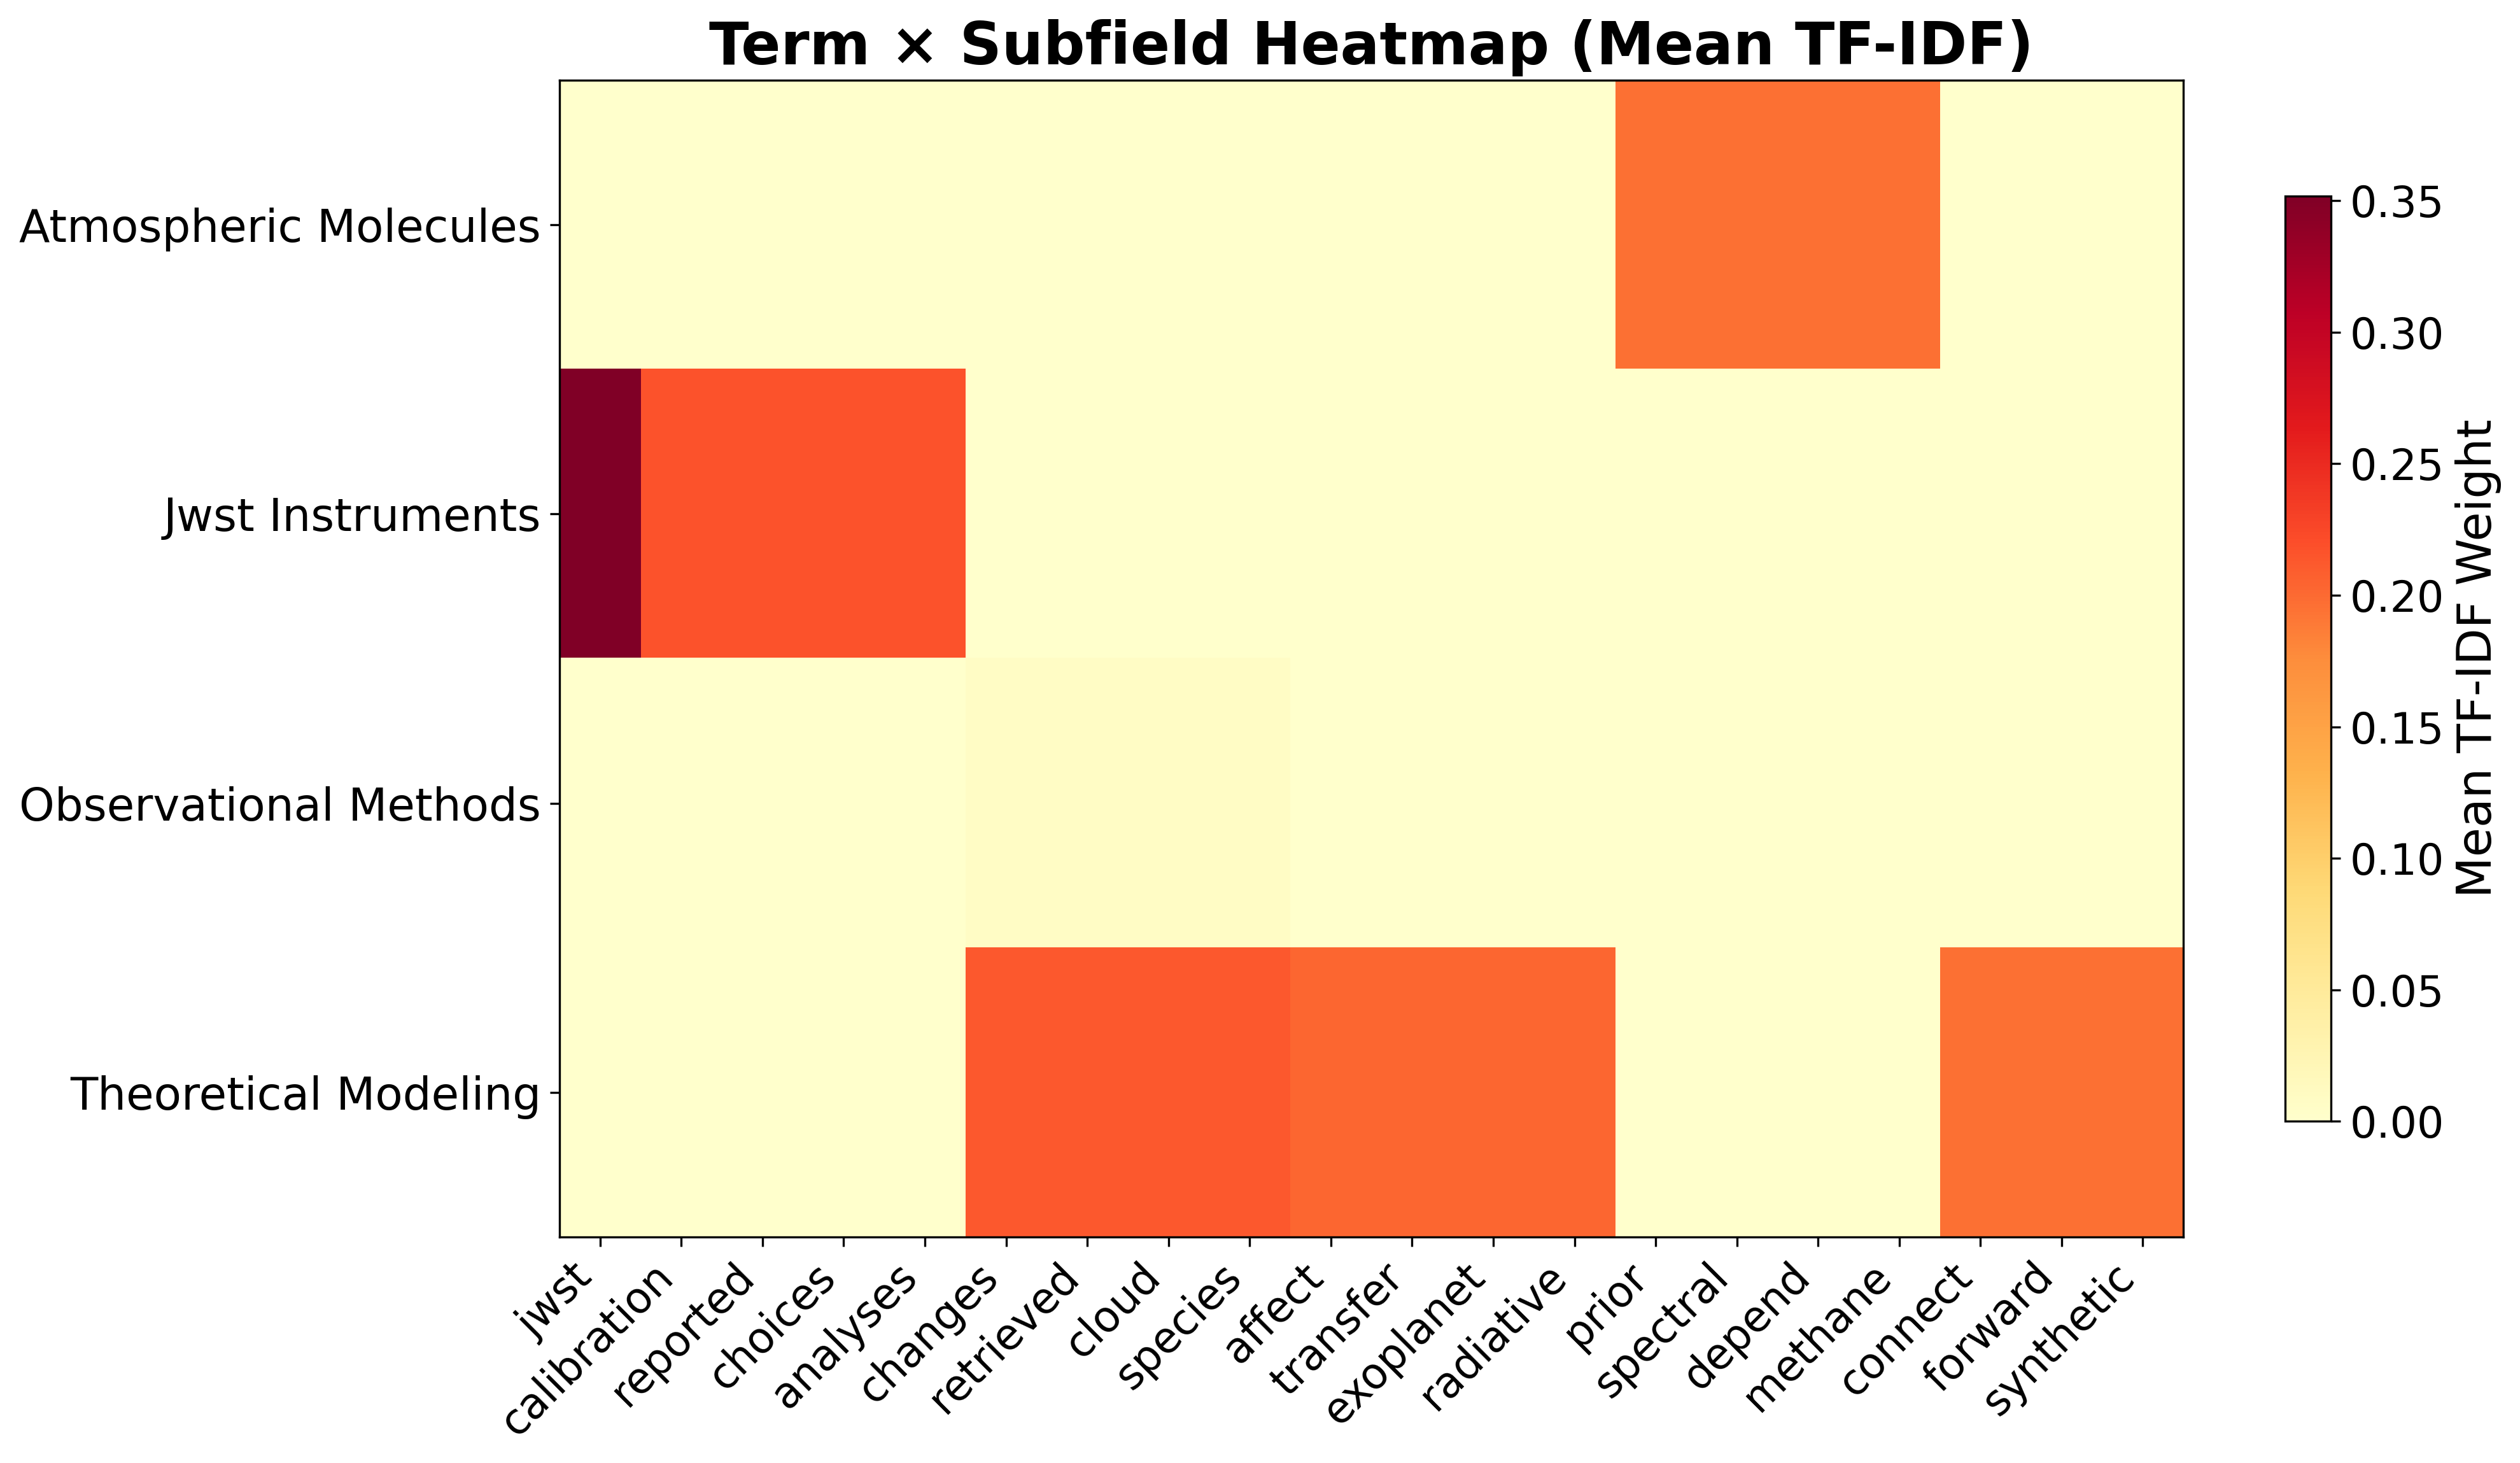
\includegraphics{../figures/term_heatmap.png}
\caption{Term heatmap for \{\{SEARCH\_TERM\_TITLE\}\}. Each cell shows
the mean TF-IDF weight of a term within a subfield. Terms are selected
by between-subfield variance to highlight discriminative vocabulary
rather than globally frequent terms.}\label{fig:term_heatmap}
\end{figure}

\newpage
\end{frame}

\begin{frame}[allowframebreaks]{Named Entity Analysis}
\phantomsection\label{named-entity-analysis}
Named entity extraction over the \{\{ABSTRACT\_COUNT\}\} abstracts
identified \{\{NUM\_ENTITIES\}\} unique entities. The most frequent
entities reflect the retained corpus and the configured extraction
rules; source coverage and fixture status determine how they may be
interpreted.

\textbf{Table 4. Top named entities in abstracts.}

\{\{TOP\_ENTITIES\_TABLE\}\}

\begin{figure}
\centering
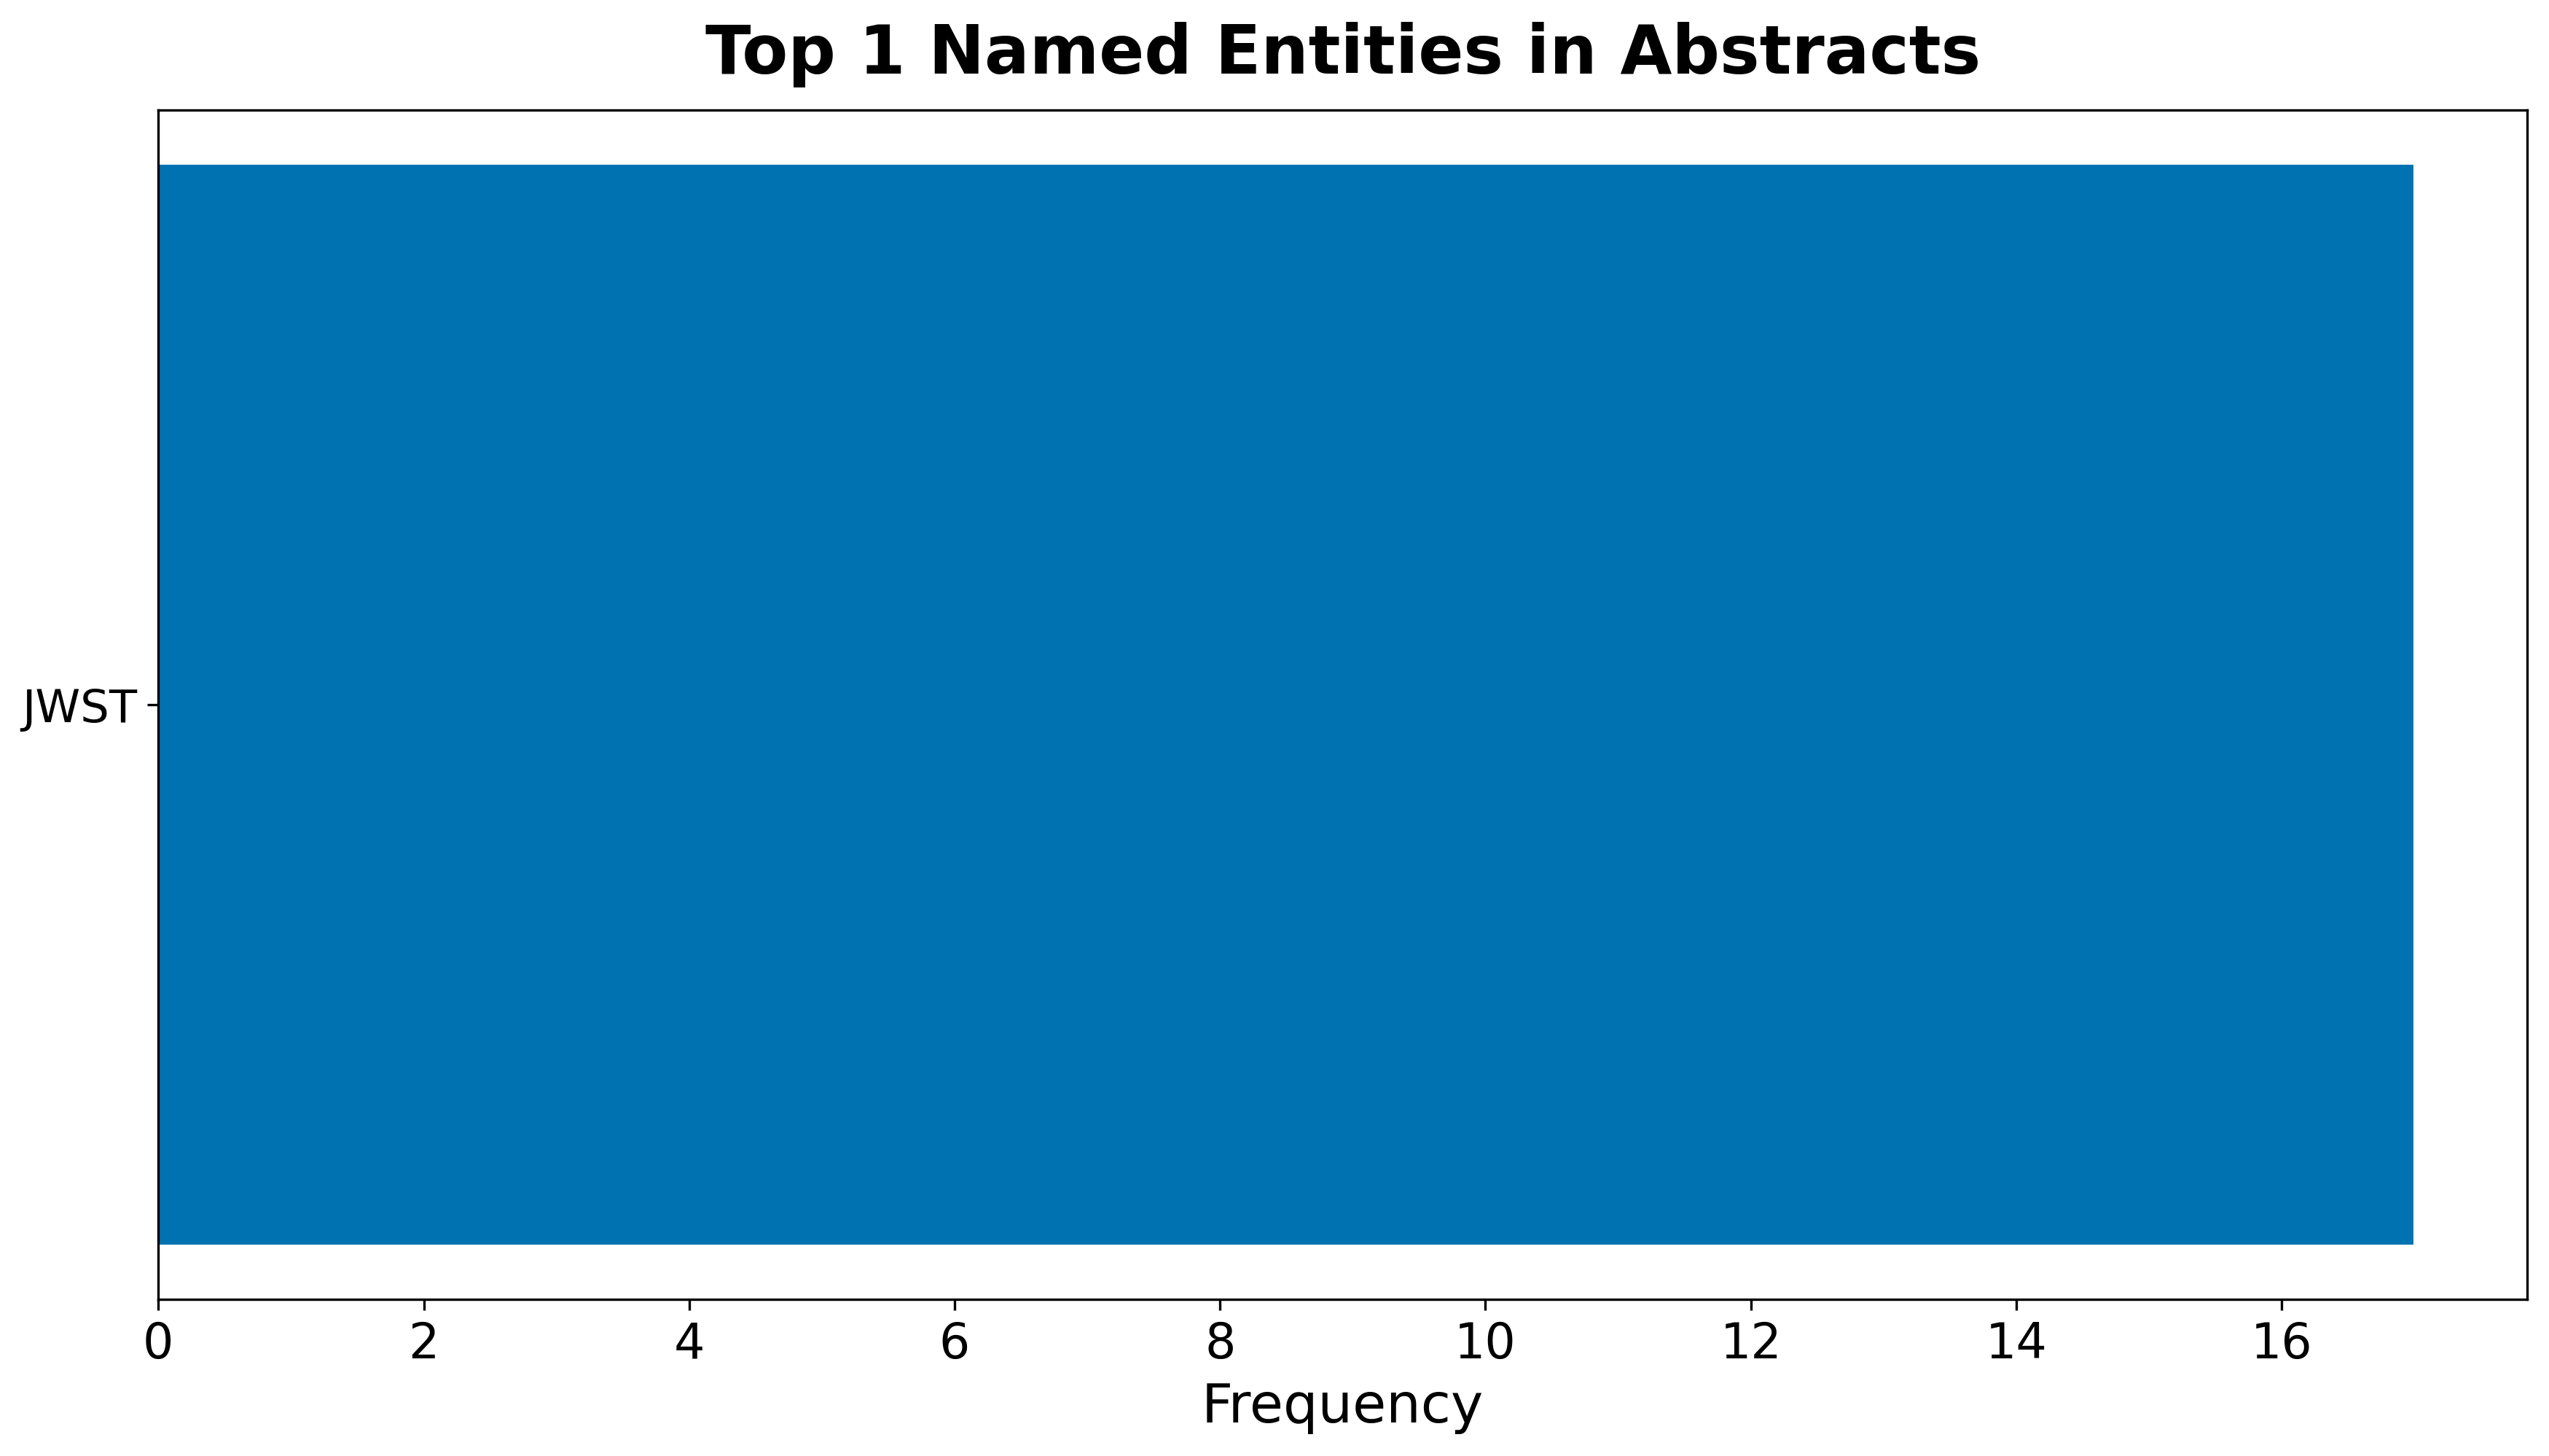
\includegraphics{../figures/entity_bar_chart.png}
\caption{Top named entities for \{\{SEARCH\_TERM\_TITLE\}\}. The
horizontal bar chart shows the 20 most frequently extracted entities
from abstracts, revealing recurring objects, instruments, methods, and
concepts in the retained corpus.}\label{fig:entity_bar_chart}
\end{figure}

\clearpage

\textbf{Table 5. Top keyphrases by TF-IDF score.}

\{\{TOP\_KEYPHRASES\_TABLE\}\}
\end{frame}

\begin{frame}[allowframebreaks]{Embedding Similarity and Clustering}
\phantomsection\label{embedding-similarity-and-clustering}
The TF-IDF/SVD embeddings place every document in a 50-dimensional
vector space. K-means clustering with \(k = {{NUM_EMBEDDING_CLUSTERS}}\)
clusters partitions the corpus into topically coherent groups. The top
similar document pairs, ranked by cosine similarity, reveal the most
closely related works in the corpus.

\textbf{Table 6. Top 10 most similar document pairs.}

\{\{TOP\_SIMILAR\_PAIRS\_TABLE\}\}

\begin{figure}
\centering
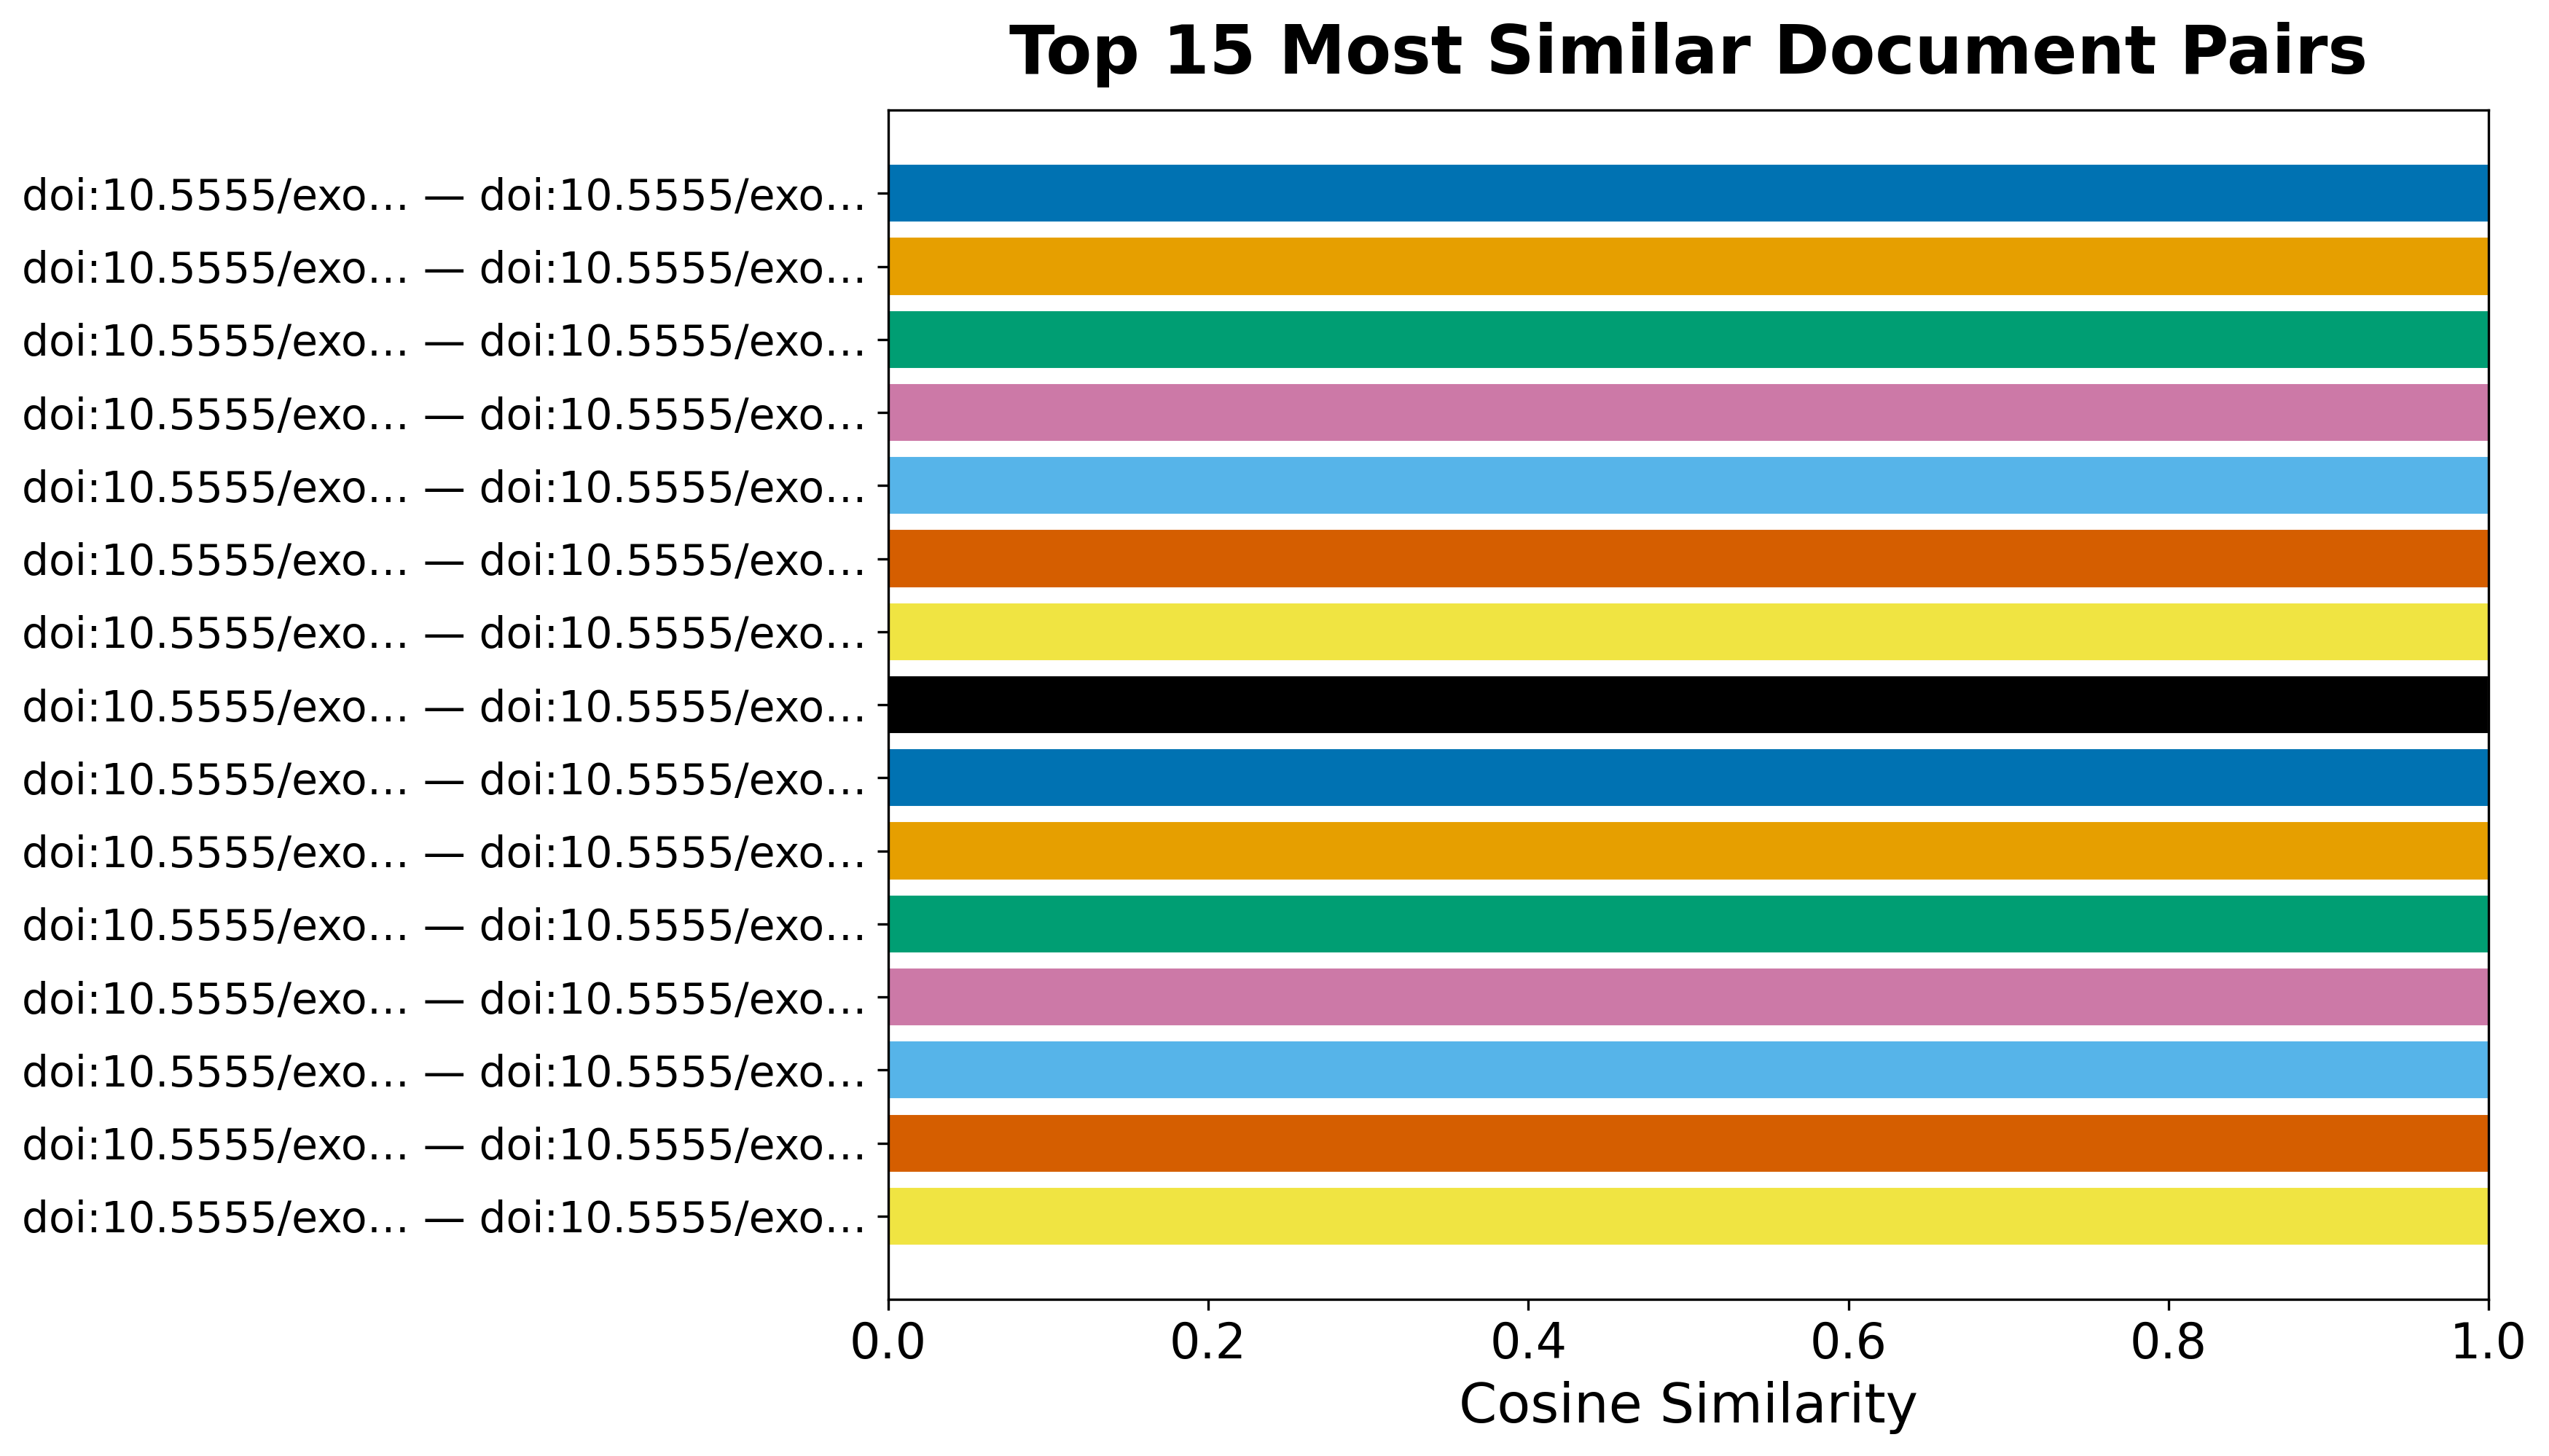
\includegraphics{../figures/similarity_heatmap.png}
\caption{Document similarity for \{\{SEARCH\_TERM\_TITLE\}\}. The
horizontal bar chart shows the 15 most similar document pairs ranked by
cosine similarity of their TF-IDF/SVD embeddings. High-similarity pairs
share topical and lexical content.}\label{fig:similarity_heatmap}
\end{figure}

\begin{figure}
\centering
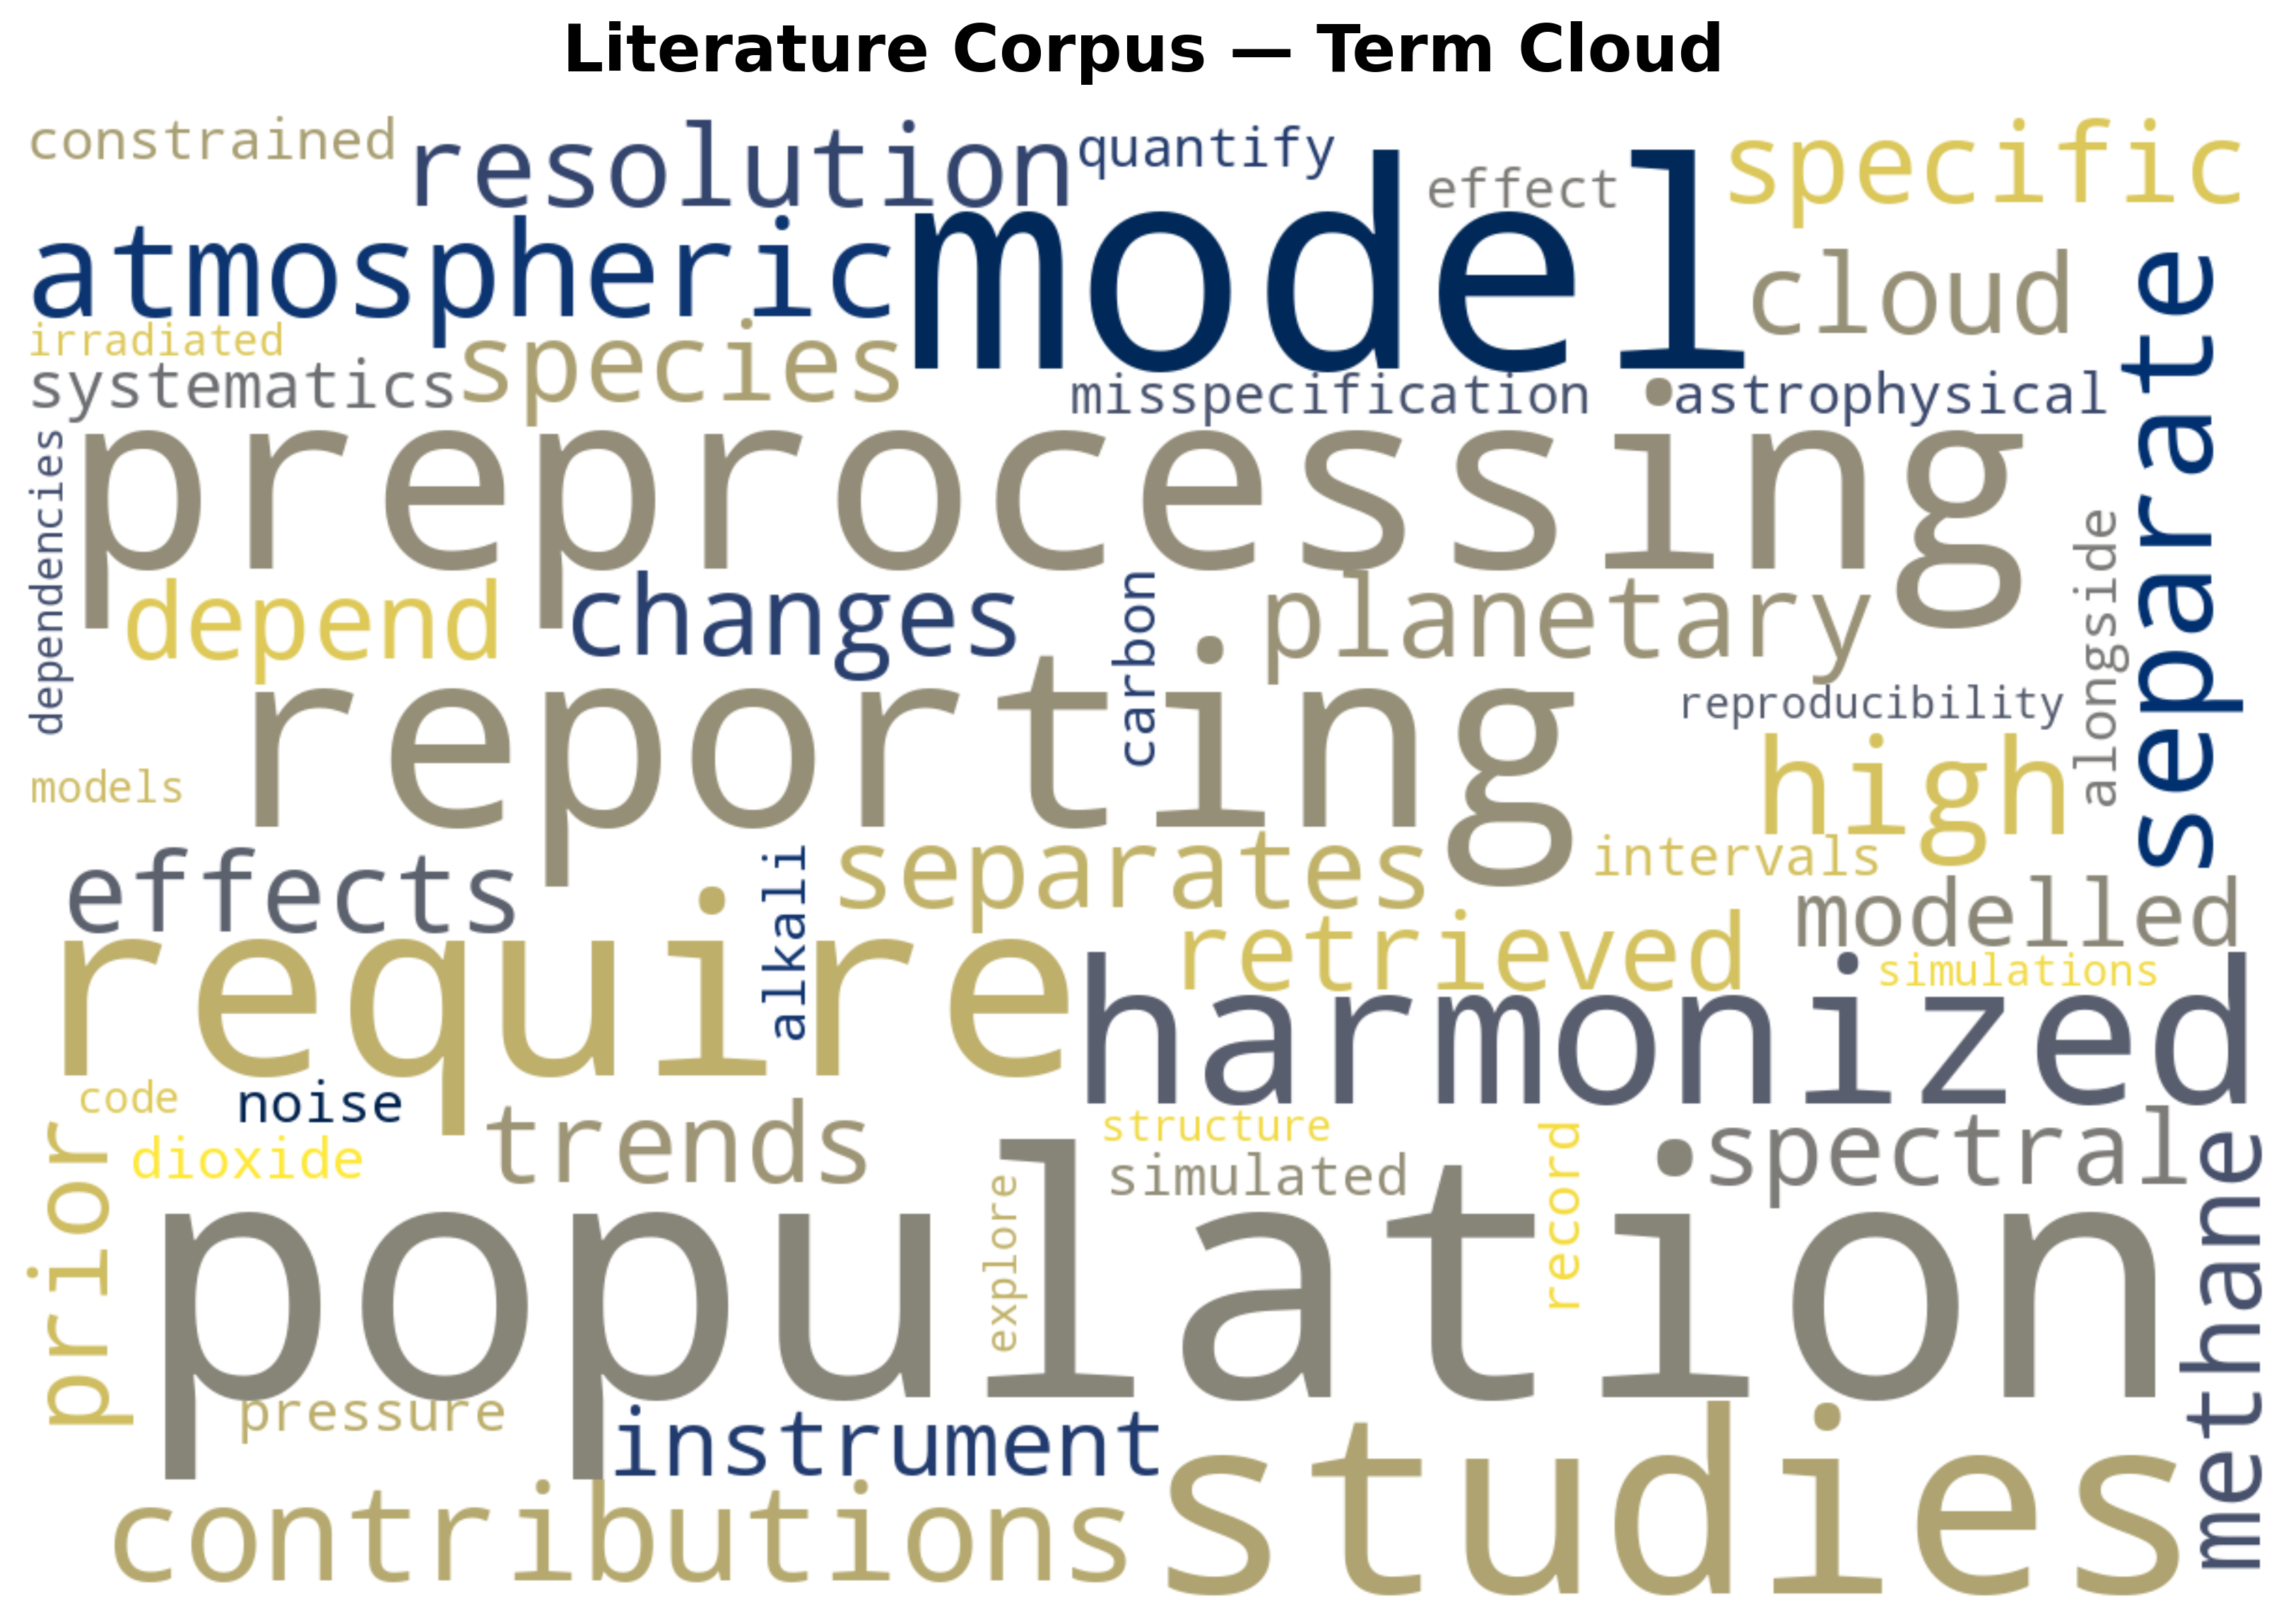
\includegraphics{../figures/word_cloud.png}
\caption{Term cloud for \{\{SEARCH\_TERM\_TITLE\}\}. Term sizes are
proportional to their TF-IDF weights across the corpus, providing a
visual summary of the dominant vocabulary.}\label{fig:word_cloud}
\end{figure}

\begin{figure}
\centering
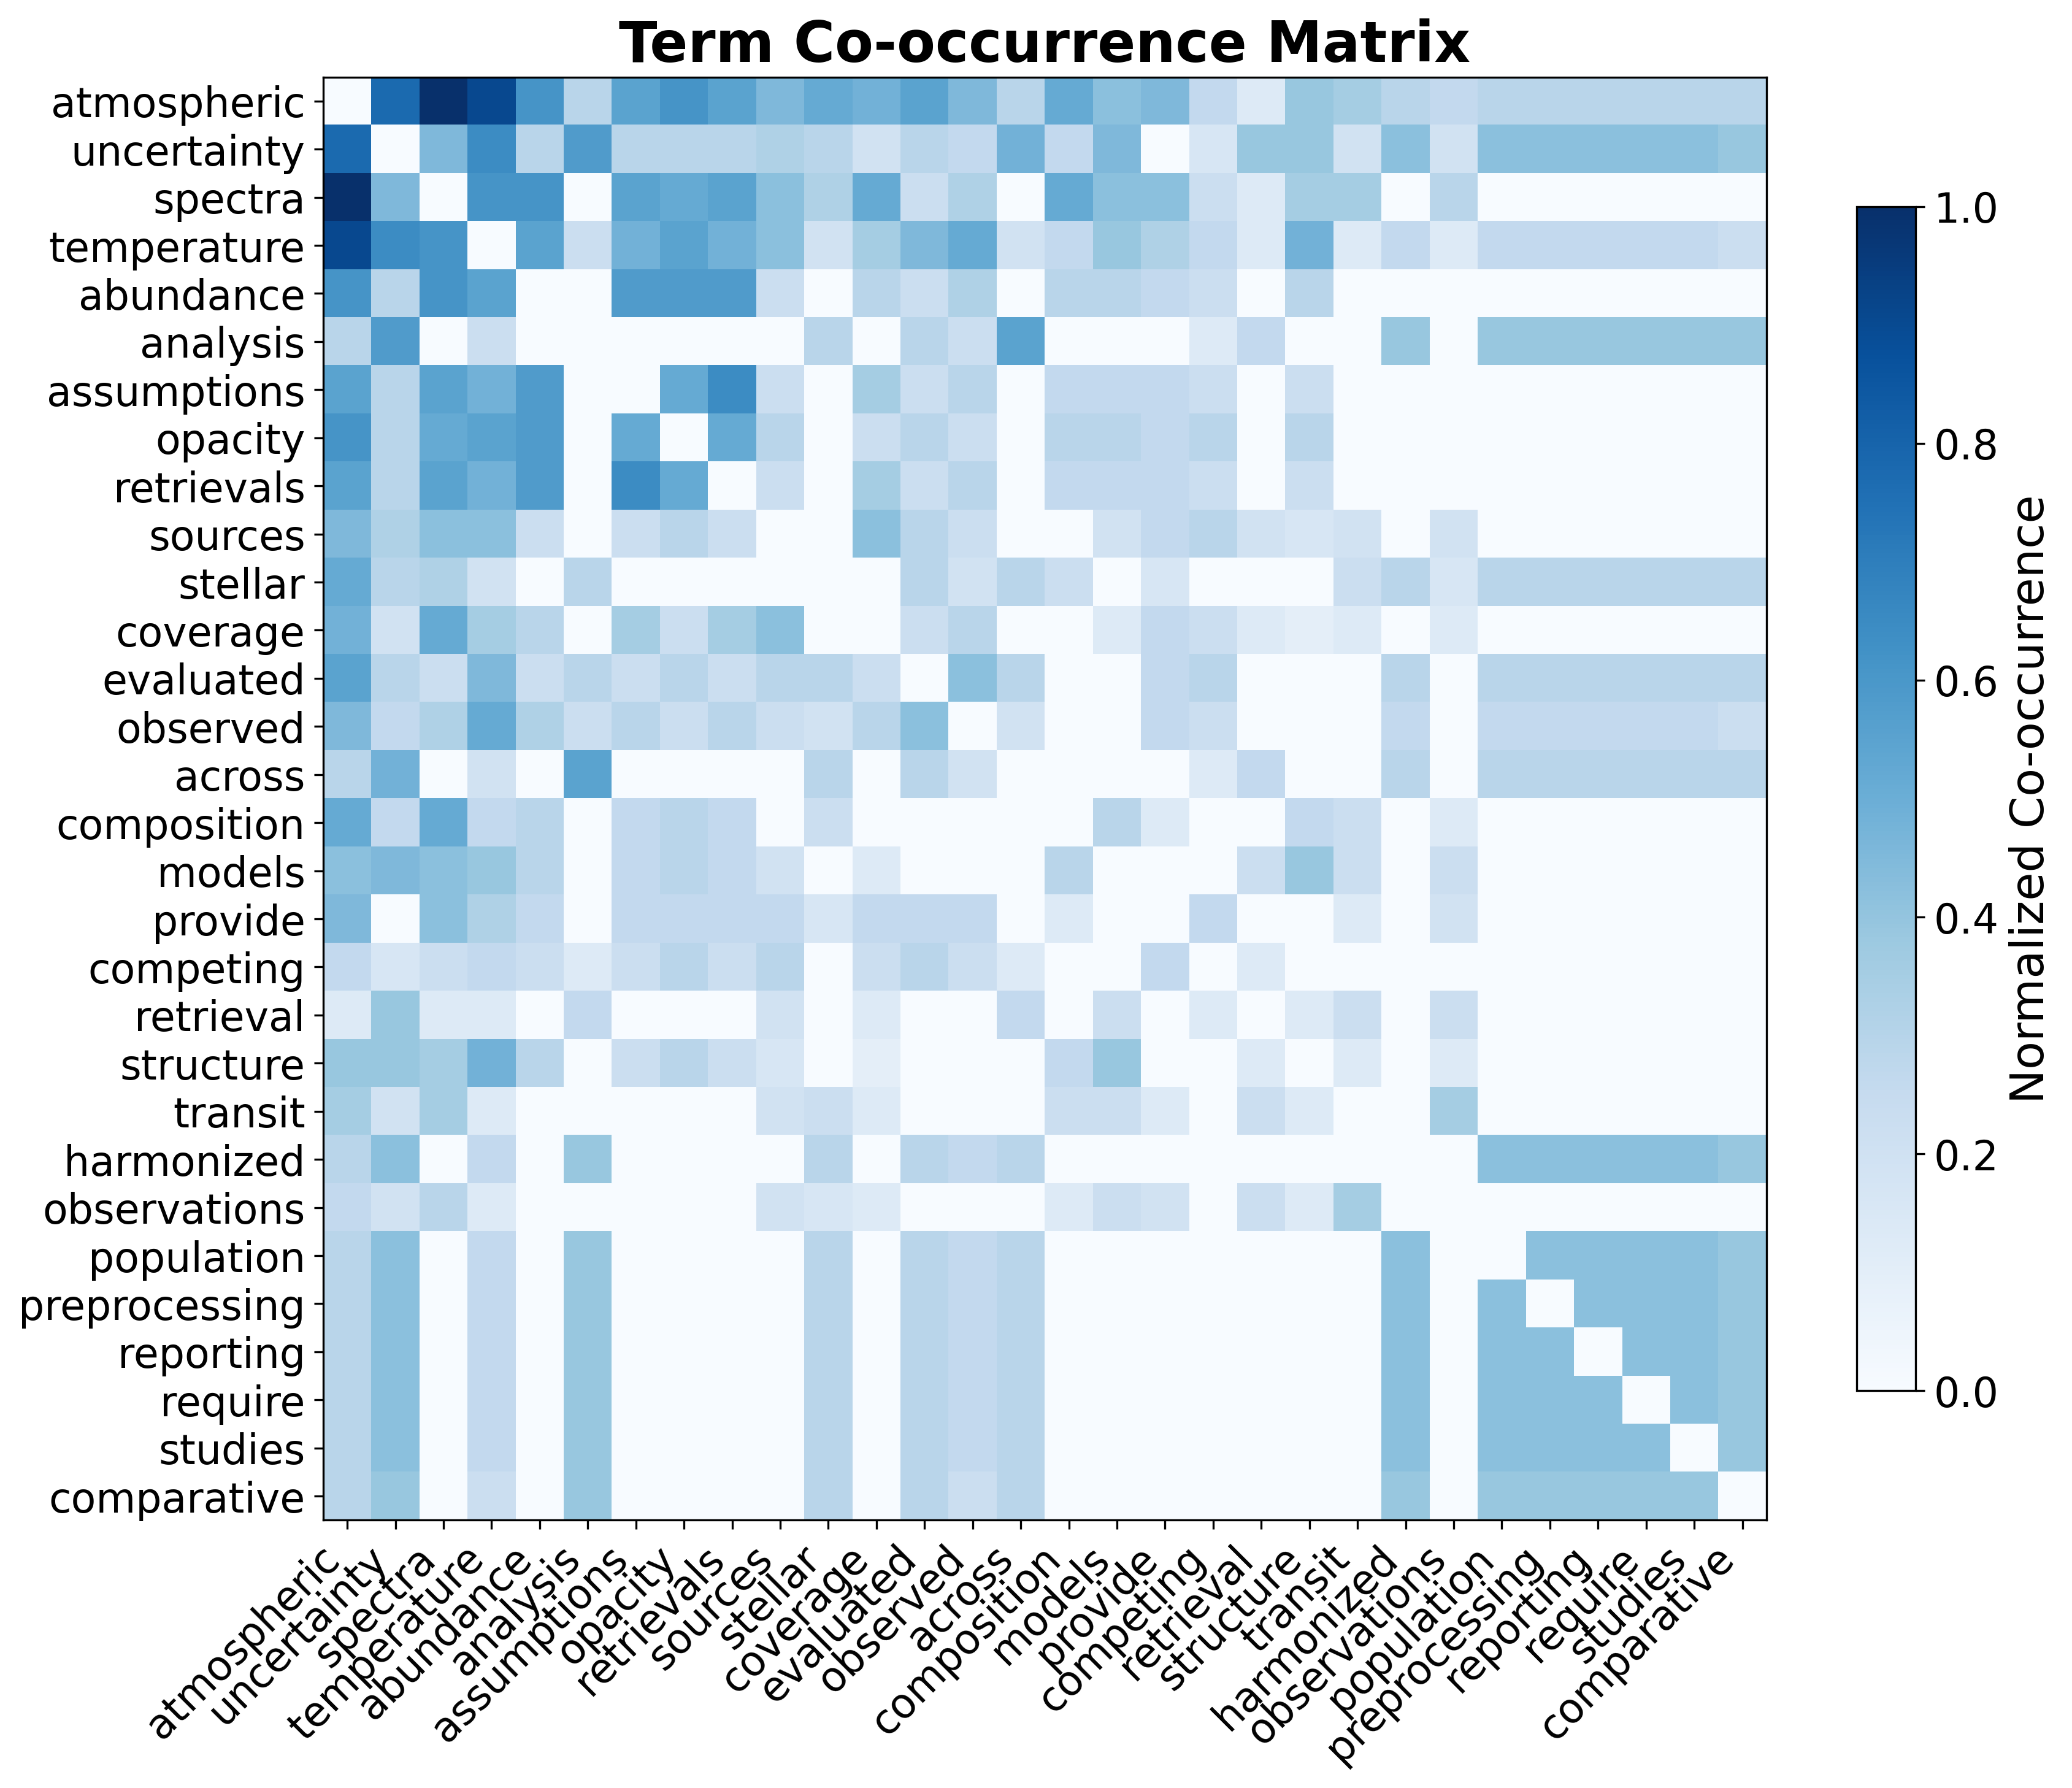
\includegraphics{../figures/cooccurrence_matrix.png}
\caption{Term co-occurrence matrix for \{\{SEARCH\_TERM\_TITLE\}\}. Each
cell shows the normalized co-occurrence frequency of two terms within
the same document, revealing which concepts tend to appear together in
the literature.}\label{fig:cooccurrence_matrix}
\end{figure}

These embeddings support semantic retrieval over the corpus and the
visual map of the literature's topical geography.
\end{frame}

\end{document}
